\documentclass[a4paper]{extarticle}
\usepackage[utf8]{inputenc}
\usepackage[a4paper, margin=1in]{geometry}

\usepackage{amssymb}
\usepackage{amsmath}
\usepackage{enumitem}
\usepackage{tcolorbox}
\usepackage{fancyhdr}
\usepackage{graphicx}
\usepackage{float}

\setlength{\parindent}{0em}
\setlength{\parskip}{0.4em}

\definecolor{theoremblue}{RGB}{1, 73, 124}
\definecolor{corollaryblue}{RGB}{70, 143, 175}
\definecolor{exampleblue}{RGB}{137, 194, 217}

\newtcolorbox{tbox}{colback=theoremblue!20,colframe=theoremblue,
boxrule=0pt,arc=0pt,boxsep=2pt,left=2pt,right=2pt,leftrule=2pt}

\newtcolorbox{cbox}{colback=corollaryblue!20,colframe=corollaryblue,
boxrule=0pt,arc=0pt,boxsep=2pt,left=2pt,right=2pt,leftrule=2pt}

\newtcolorbox{ebox}{colback=exampleblue!20,colframe=exampleblue,
boxrule=0pt,arc=0pt,boxsep=2pt,left=2pt,right=2pt,leftrule=2pt}

\title{EnpRisk - Lecture Notes Week 4}
\author{Ruben Schenk, ruben.schenk@inf.ethz.ch}
\date{\today}

\pagestyle{fancy}
\fancyhf{}
\rhead{ruben.schenk@inf.ethz.ch}
\rfoot{Page \thepage}
\lhead{EnpRisk - Lecture Notes Week 4}

\begin{document}

\maketitle
\newpage

\subsubsection{Relative Valuation}

In \textbf{relative valuation,} the valuation of an asset is deduced from the market value of a set of similar assets. To do relative valuation:

\begin{itemize}
    \item We need to identify comparable assets and obtain their market value
    \item Standardize these market values, because absolute prices cannot be compared
\end{itemize}

This process of standardization creates \textbf{valuation multiples} (price multiples):

\begin{itemize}
    \item \textbf{P/E ratio:} Calcualte a company's share price (Equity) from its earnings (net profit)
    \item \textbf{EV/EBITDA ratio:} Calculate a company's enterprise value from its EBITDA
    \item \textbf{EV/EBIT ration:} Calcualte a company's enterprise value from its EBIT
\end{itemize}

\subsubsection{Cash Flow Statement}

The components of the \textbf{cash flow statement} can be categorized into three different groups:

\begin{itemize}
    \item Operating Activities = Net Income - Non Cash Expenses - Increase in Working Capital
    \item Investing Activities = Purchases/Sale of long term assets (\textit{Capex}) + Purchase/Sale of other business (\textit{M\&A}) + Purchase/Sale of marketable securities
    \item Financing Activities = Issue/Repurchase equity + Issue/Repruchase debt + Dividend payments and other items
\end{itemize}

The \textit{change in working capital} \(\delta WC\) = Change in accounts receivable + changein inventory - change ina ccounts payable, where the \textit{accounts receivable} is the sume of all invoices send out to customers that have not been paid yet, and \textit{accounts receivable} is the sum of all invoices received from vendors that you have not paid yet.

\begin{ebox}
    \textbf{Example:} Consider the following table displaying the cash and cash flow from our taxi business:

    \begin{figure}[H]
        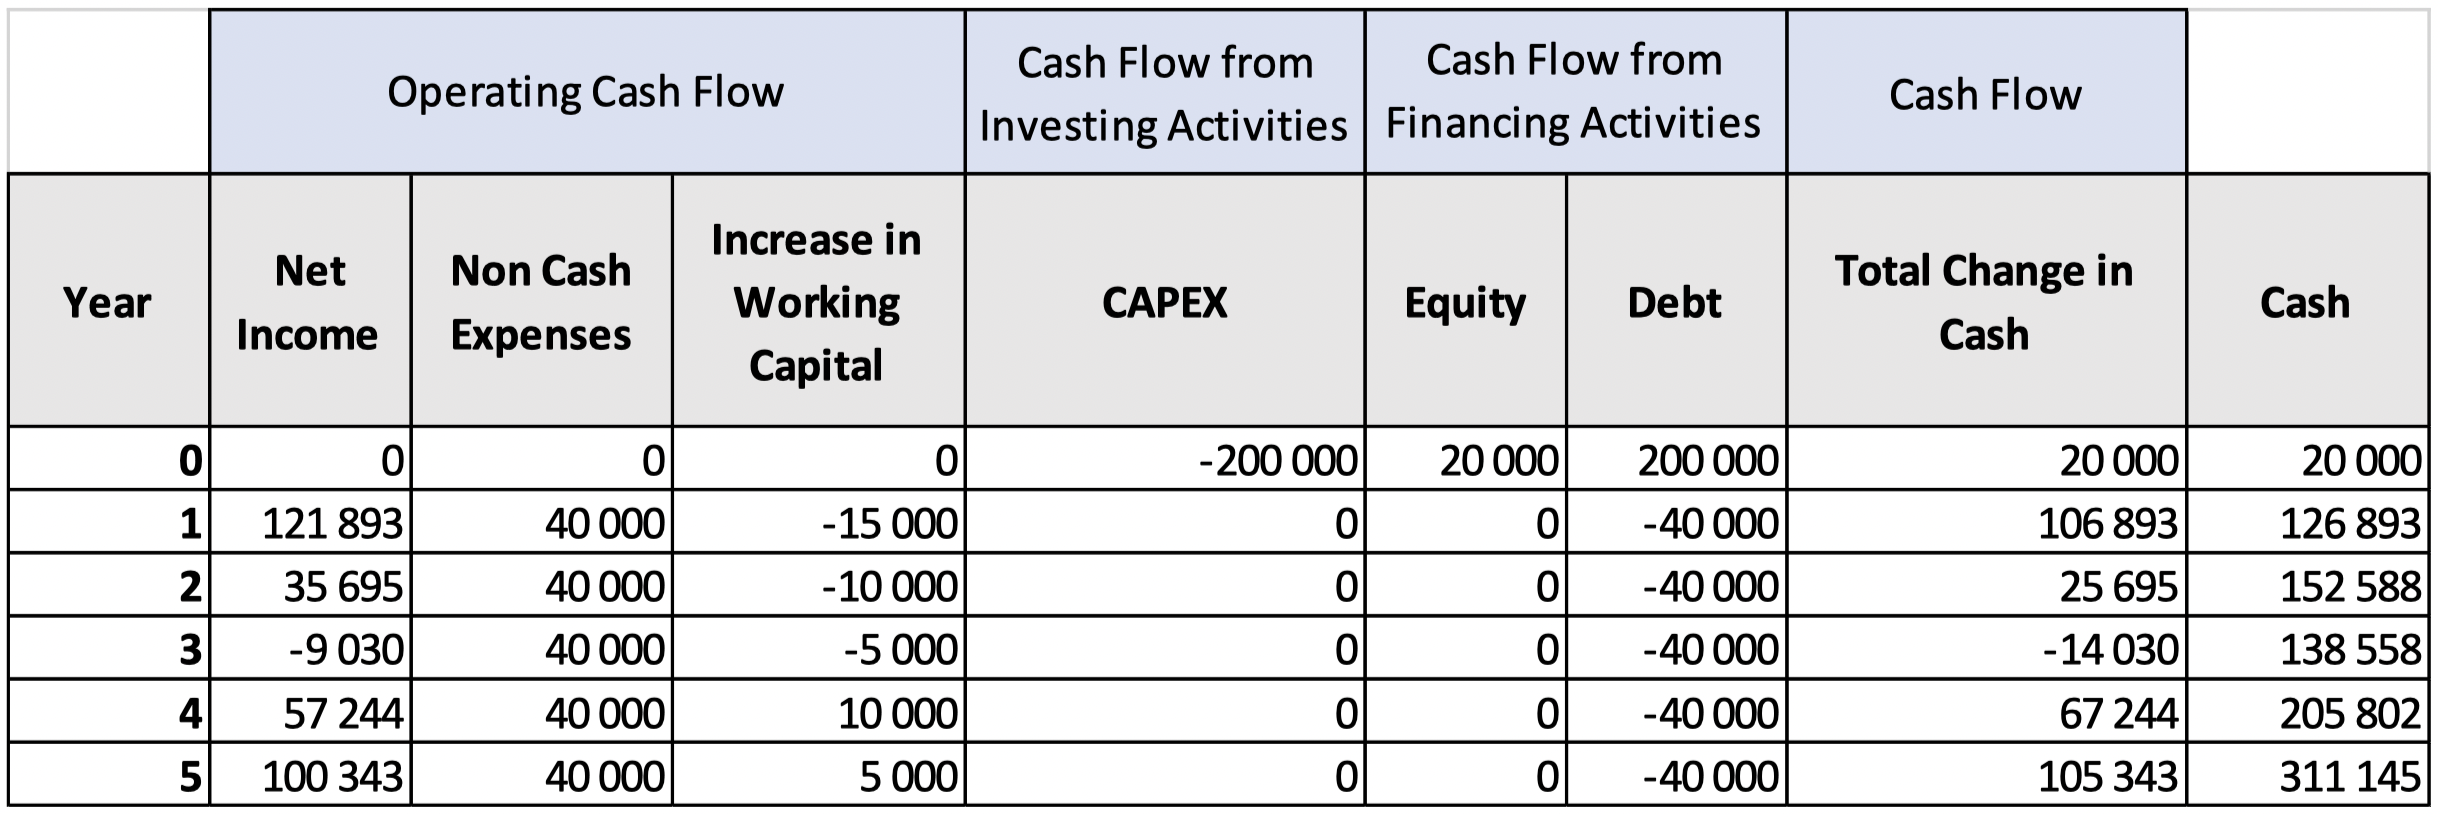
\includegraphics[width=15cm]{../images/EnpRisk_Fig4-1}
        \centering
    \end{figure}
\end{ebox}

\paragraph{Discounted Cash Flow Valuation} One might also value a company with the \textbf{time value of money.} It is given by the following formula:

\[
    FV = PV \times (1 + r)^n,
\]
where \(FV\) is the future value, \(PV\) is the present value, \(r\) is the rate of return (or discount rate), and \(n\) is the number of periods.

The principle of time value of money is used to calculate the \textbf{price of a bond.} The formula is as follows:

\[
    Bond \, Price = \frac{C}{(1 + i)} + \frac{C}{(1 + i)^2} + \cdots + \frac{C}{(1 + i)^n} + \frac{M}{(1 + i)^n},
\]
where \(C\) is the coupon payment, \(n\) is the number of payments, \(i\) is the interest rate, and \(M\) is the value at maturity (or par value).

We may also use this formula to value a mature business with cash flow growing steadily at \(g\):

\begin{align*}
    &PV = \sum_{i = 1}^{\infty} \frac{CF_i}{(1 + r)^i} \Rightarrow PV = \sum_{i = 1}^{\infty} \frac{CF_0[1 + g]^i}{(1 + r)^i} \\
    &PV = CF_0r' \sum_{i = 0}^{\infty} r'^i \Rightarrow PV = CF_0 \frac{r'}{1 - r'} \\
    &PV = CF_0 \frac{1 + g}{r - g} \Rightarrow PV = \frac{CF_1}{r - g} \\
    &\frac{PV}{CF_1} = \frac{1}{r - g} \Rightarrow r = \frac{CF_1}{P} + g
\end{align*}
where \(r' = \frac{1 + g}{1 + r}\). This is called the \textbf{dividend discount model} or the \textit{Gordon-Shapiro formula:} The total return is divident yield plus the growth rate.

\subsubsection{Summary: Three Ways of Valuation}

The \textit{balance sheet evaluation} gives you the company's \textbf{book value,} that is its shareholders' equity (capital and reserves), or the difference between its assets and liabilities. This doesn not take into cosnideration the fact that a company is a \textit{little machine} or a \textit{process} that generates profit based on people, proesses, and stuff.

If you buy a company, you buy a little profit-making machine. So it makes sense to use porift generation as a basis in the valuation. That is when you do \textbf{relative valuation} based on market-calibrated multiples and different metrics in the \textit{P\&L}, e.g. EBITDA, EBIT, net profit etc.

However, this supposes that the company is in a sort of steady state or dynamic equilibrium. For a growth company, earnings will increase in the future and so will its valuation.

For companies that are structured for growth, the \textbf{discounted cash flow} approach is needed.

\subsubsection{Bubble Model}

The standard model for bubbles is given by the \textbf{Geoemtric Brownian Motion:}

\begin{figure}[H]
    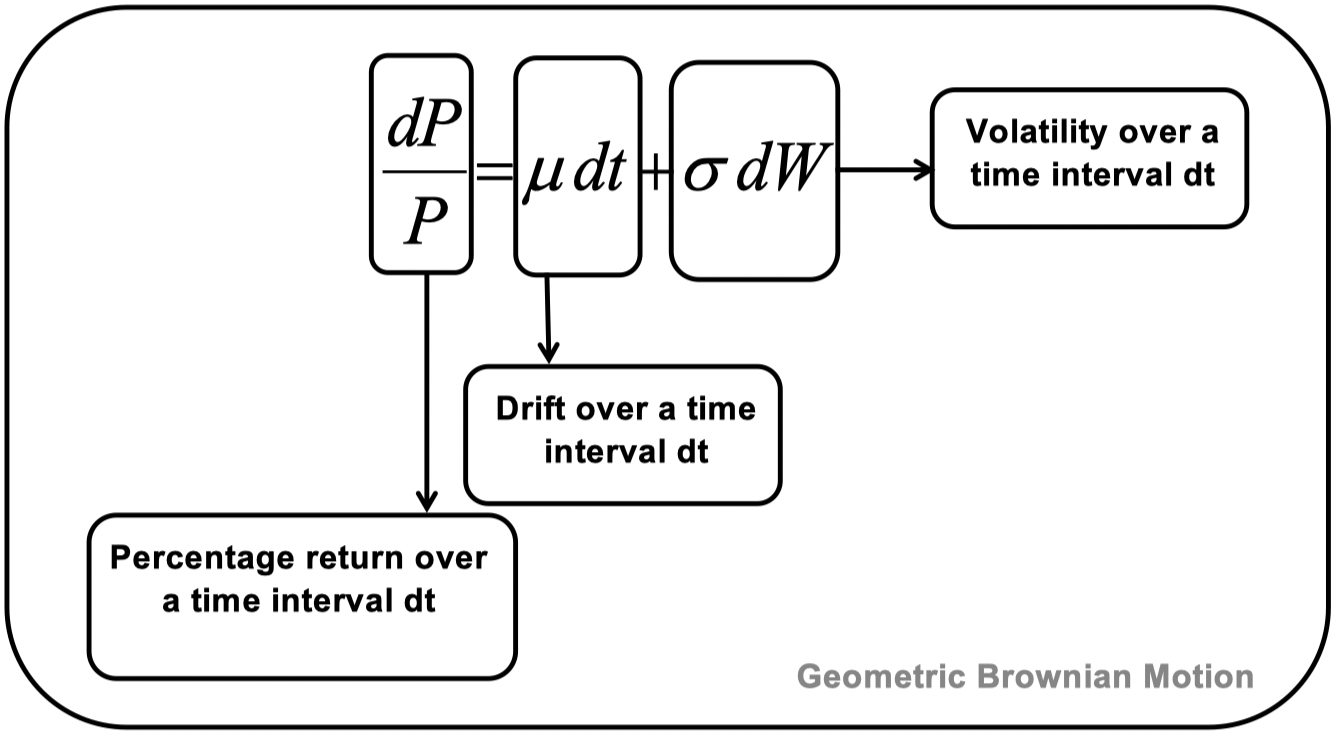
\includegraphics[width=9cm]{../images/EnpRisk_Fig4-2}
    \centering
\end{figure}

The standard GBM, without noise, is basically given by an exponential function:

\[
    \frac{dP}{P} = \mu dt \Rightarrow \frac{d\log P}{dt} = \mu.
\]

When we add feedback, the growth rate is no longer constant but increases with the price, for example:

\[
    \frac{d \log P}{dt} = \mu [P] \simeq P^{\delta}.
\]

During such phases, the market is in a \textbf{bubble} - the growth rate increases with the price, there is positive feedback.

We can describe a bubble as follows:

\begin{itemize}
    \item A bubble starts with a new opportunity or expectation
    \item Smart money flows in, which leads to a first price appreciation
    \item Attracted by the prospect of higher returns, less sophisticated investors follow
    \item Demand goes up as the price increases, and the price goes up as the demand increases. This creates a positive feedback machanism. The market is fully driven by behavior and sentiment and no longer reflects any real underlying value.
\end{itemize}

The crash can be described in the following way:

\begin{itemize}
    \item At some point. investors start realizing that the process is no longer sustainable and the market collapses.
    \item The crash occurs because the market has entered an unstable phase.
    \item This mechanism is often not well understood, and a great controversy rises about the cause of the crash.
\end{itemize}

\subsubsection{Intuition behind Complex Systems}

Complex does not mean complicated, it has a very specific meaning! A \textbf{complex system:}

\begin{itemize}
    \item Consists of a large ensemble of agents, like molecuels, stars, insects, etc.
    \item These interact, e.g. they may repel, attract or imitate each other
\end{itemize}

However, having a large set of interacting agents is not enough. A system is said to be "complex", when there is \textbf{emergence,} that is, when localinteractions lead to global cooperation, in absence of any global orchestration.

Without any external coordination, an audience can applaud synchronously. This is the result of interaction of epople, they start imitating until finally a global synchornization sets in.

It can be surprising, but synchronous applause has much in common with financial bubbles and crashes.

\end{document}